\section{Công nghệ sử dụng}
\subsection{Front-end: React.js và Vite}
React.js đảm nhiệm tầng trình diễn (presentation layer) của thư viện trực tuyến, xây dựng giao diện tương tác cho tìm kiếm, duyệt sách, và trò chuyện với trợ lý AI. Vite được sử dụng làm công cụ build/dev server để khởi động nhanh, hỗ trợ HMR và tối ưu hóa bundle cho môi trường production. Trên client, các component chịu trách nhiệm: hiển thị kết quả tìm kiếm (kết hợp highlight từ semantic matches), quản lý trạng thái người dùng (cache, optimistic updates), và tích hợp SDK cho chat/assistant (streaming responses, conversation state).
\begin{figure}[htbp]
\centering
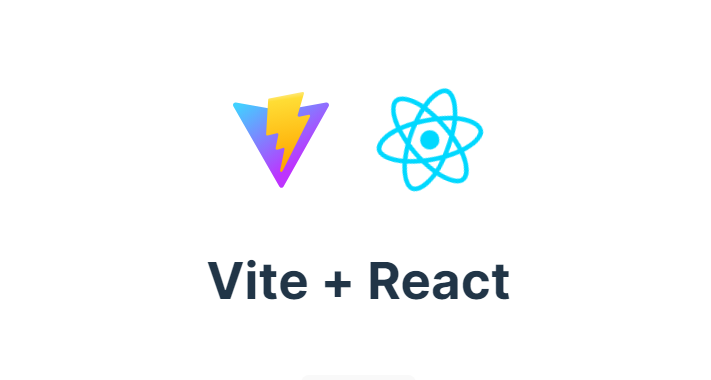
\includegraphics[width=0.4\textwidth]{Images/react_vite.png}
\end{figure}

\subsection{Back-end: Node.js và Express}
Node.js + Express cung cấp API REST/GraphQL chính cho chức năng quản lý sách, người dùng, và phiên làm việc. Server này thực hiện điều phối yêu cầu: xác thực/RBAC, điều khiển transaction với PostgreSQL qua Prisma, và ủy nhiệm các tác vụ AI (tạo embedding, tóm tắt, truy vấn RAG) tới dịch vụ AI chuyên trách. Đặt các endpoint chuẩn hóa cho search, recommendation, và webhook tích hợp (ví dụ cập nhật metadata từ Open Library).
\begin{figure}[htbp]
\centering

\includegraphics[width=0.4\textwidth]{Images/node_express.jpg}
\end{figure}

\subsection{Dịch vụ AI chuyên trách: Python và FastAPI}
Dịch vụ AI tách biệt (microservice) được hiện thực bằng Python + FastAPI để tận dụng thư viện NLP/ML (transformers, sentence-transformers, hay client SDK của nhà cung cấp LLM). Nhiệm vụ: sinh embedding, làm tóm tắt tài liệu, trả lời QA qua RAG, và xử lý pipeline tiền/thuật toán (prompt engineering, chunking, reranking). FastAPI phù hợp cho endpoints đồng thời thấp-latency và dễ mở rộng theo nhu cầu tải.
\begin{figure}[htbp]
\centering

\includegraphics[width=0.4\textwidth]{Images/fastapi.png}
\end{figure}

\subsection{ORM: Prisma}
Prisma (TypeScript) được dùng để định nghĩa schema, sinh client truy vấn và quản lý migration cho PostgreSQL. Prisma giúp duy trì kiểu an toàn giữa ứng dụng Node và cơ sở dữ liệu, đơn giản hóa các truy vấn liên quan đến mượn–trả, lịch sử giao dịch, và metadata sách; đồng thời hỗ trợ transaction khi cần đảm bảo tính nhất quán (ACID).
\begin{figure}[htbp]
\centering

\includegraphics[width=0.4\textwidth]{Images/prisma.png}
\end{figure}

\subsection{Cơ sở dữ liệu quan hệ: PostgreSQL}
PostgreSQL lưu trữ dữ liệu quan hệ chính: bản ghi sách, người dùng, giao dịch mượn, và metadata. Lợi thế: tuân thủ ACID cho quy trình mượn–trả, hỗ trợ các tính năng nâng cao (JSONB cho metadata linh hoạt, full-text search cho chỉ mục từ khóa) và khả năng mở rộng bằng replication/partitioning khi cần.
\begin{figure}[htbp]
\centering
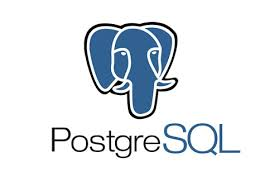
\includegraphics[width=0.4\textwidth]{Images/postgresql.jpg}
\end{figure}

\subsection{Vector DB và Embeddings: pgvector / Vector store}
Embedding vectors cho nội dung sách (toàn văn, đoạn tóm tắt) được lưu trong `pgvector` (mở rộng PostgreSQL) hoặc một vector database chuyên dụng. Vector store cho phép thực hiện nearest-neighbor searches (cosine similarity) để hỗ trợ tìm kiếm ngữ nghĩa, truy xuất ngữ cảnh cho RAG, và tính năng "similar books" trong recommendation. Thiết kế lưu trữ kèm metadata để nhanh chóng map vector về tài liệu gốc.

\subsection{AI / LLM: Embeddings, RAG, Tóm tắt và Chatbot}
Hệ thống tích hợp LLM cho nhiều chức năng: tạo embedding cho semantic search, kết hợp RAG để trả lời câu hỏi dựa trên nội dung sách, tóm tắt chương/đoạn để hiển thị preview, và xây dựng chatbot hỗ trợ tra cứu tài liệu. Kiến trúc an toàn dùng prompt-template có kiểm soát, cache kết quả embedding, và cơ chế fallback/attribution khi LLM trả lời dựa trên nguồn cụ thể.
\begin{figure}[htbp]
\centering
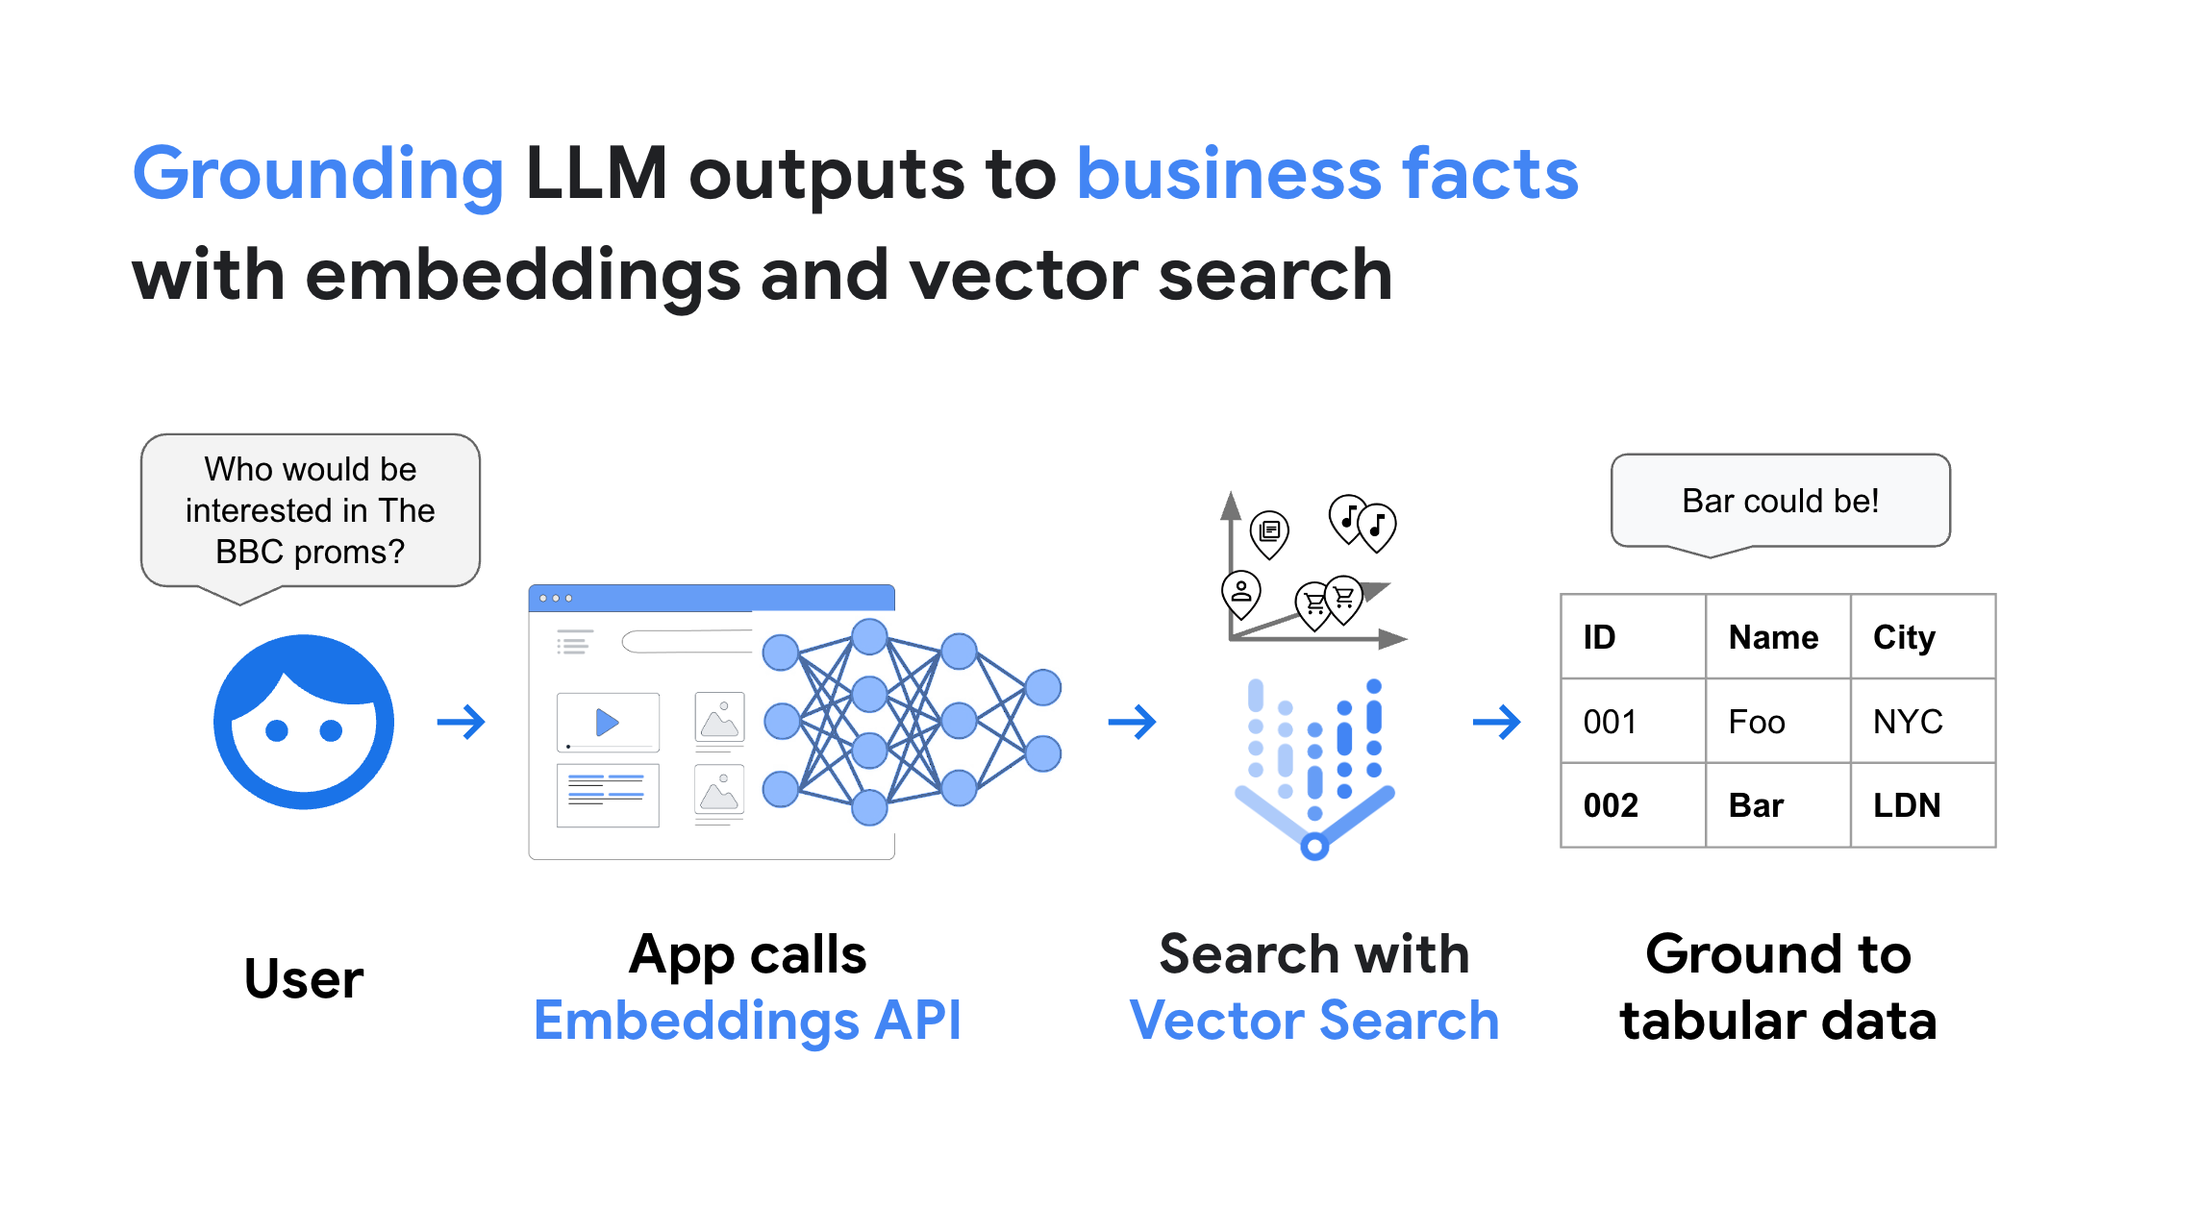
\includegraphics[width=0.5\textwidth]{Images/EmbeddingsAPI.png}
\end{figure}

\subsection{Tìm kiếm lai (Hybrid Search)}
Triển khai tìm kiếm lai tổng hợp: 1) full-text / keyword search trên PostgreSQL để hỗ trợ truy vấn chính xác theo metadata và từ khóa; 2) vector search trên pgvector để hỗ trợ truy vấn ngữ nghĩa và truy xuất theo ngữ cảnh. Kết quả được hợp nhất và rerank (ví dụ dựa trên relevance score, popularity, hoặc user context) trước khi trả về cho client.

\subsection{Bảo mật và Xác thực: JWT, RBAC, OTP}
Hệ thống sử dụng JWT để quản lý phiên người dùng và refresh token cho giữ đăng nhập an toàn. RBAC định nghĩa quyền cho vai trò (admin, librarian, member) với kiểm tra tại gateway/endpoint. OTP (email/SMS) được dùng cho xác thực hai bước quan trọng (mượn sách, thay đổi thông tin). Các biện pháp khác: HTTPS/TLS, rate limiting, logging/audit cho hành vi quan trọng.

\subsection{Tích hợp bên ngoài: Open Library / Google Books / Nodemailer}
Open Library / Google Books API dùng để tự động hóa thu thập metadata, bìa sách và thông tin xuất bản theo ISBN; quy trình ETL định kỳ kiểm tra và cập nhật metadata. `Nodemailer` (hoặc dịch vụ SMTP/Transactional) chịu trách nhiệm gửi thông báo (nhắc trả sách, reset mật khẩu, thông báo hệ thống) với template có khả năng nội dung động và log gửi.
\begin{figure}[htbp]
\centering

\includegraphics[width=0.3\textwidth]{Images/Google-play-book-icon.png}
\end{figure}

 